\section*{Protocol state machines design}
In this section we will explain, on a high abstraction level, what the protocol state machines does.
\subsection*{Webserver - Enterprise protocol}
\begin{figure}
\centering
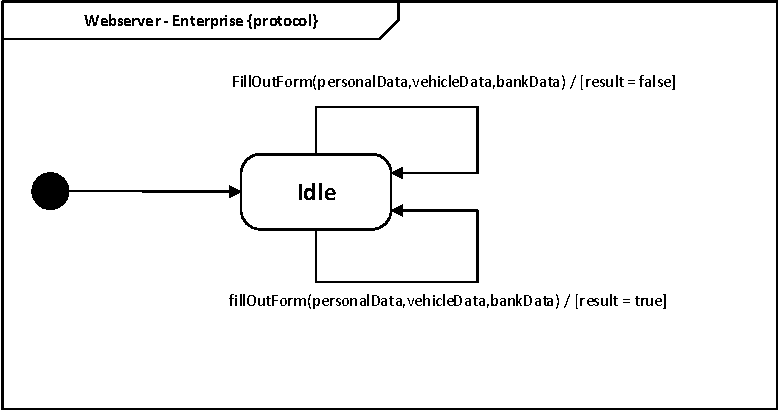
\includegraphics[width=0.7\linewidth]{img/protocol_state_machine/protocol_state_machine_webserver_to_enterprise.png}
\caption{The communication protocol for buying toll tags}
\label{fig:protocol_state_machine_webserver_to_enterprise}
\end{figure}

\subsection*{Touchscreen protocol}
\begin{figure}
\centering
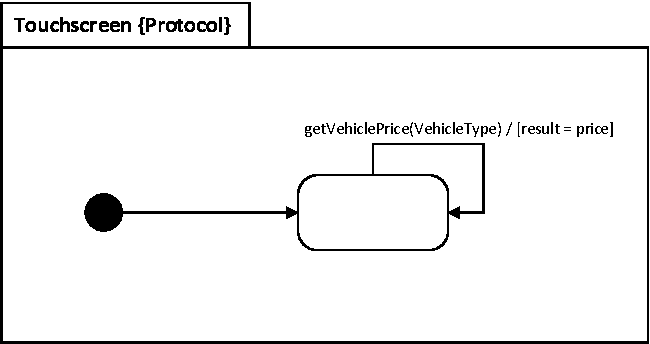
\includegraphics[width=0.7\linewidth]{img/protocol_state_machine/protocol_state_machine_touchscreen.png}
\caption{Protocol statemachine for the touchscreen}
\label{fig:protocol_state_machine_touchscreen}
\end{figure}
The diagram in \autoref{fig:protocol_state_machine_touchscreen} shows the communication protocol for getting the price for different vehicle types. It's used by customers if it is a credit card lane, and the cashier if it is a cash lane.

\subsection*{Antenna protocol}
\begin{figure}
\centering
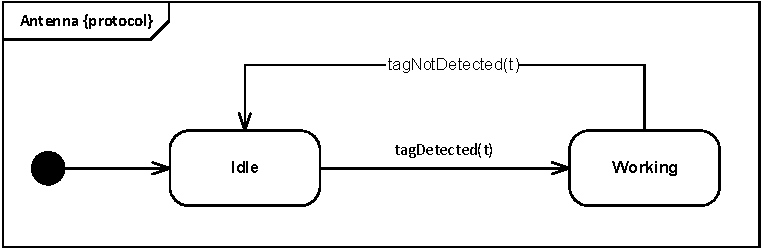
\includegraphics[width=0.7\linewidth]{img/protocol_state_machine/protocol_state_machine_antenna.png}
\caption{The interface the antenna uses, to send out messages when cars are detected}
\label{fig:protocol_state_machine_antenna}
\end{figure}

\subsection*{Credit card reader protocol}
\begin{figure}
\centering
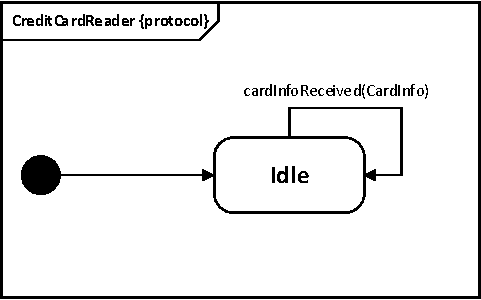
\includegraphics[width=0.7\linewidth]{img/protocol_state_machine/protocol_state_machine_tlc_to_ccr.png}
\caption{The interface for sending data about credit card information}
\label{fig:protocol_state_machine_tlc_to_ccr}
\end{figure}

\subsection*{Toll lane - bank protocol}
\begin{figure}
\centering
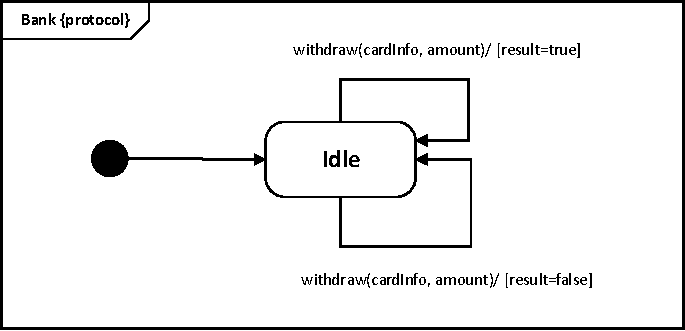
\includegraphics[width=0.7\linewidth]{img/protocol_state_machine/protocol_state_machine_tlc_to_bank.png}
\caption{Communications protocol between the bank and the credit card toll lane is shown}
\label{fig:protocol_state_machine_tlc_to_bank}
\end{figure}

\subsection*{Station server - normal toll lane checkout}
\begin{figure}
\centering
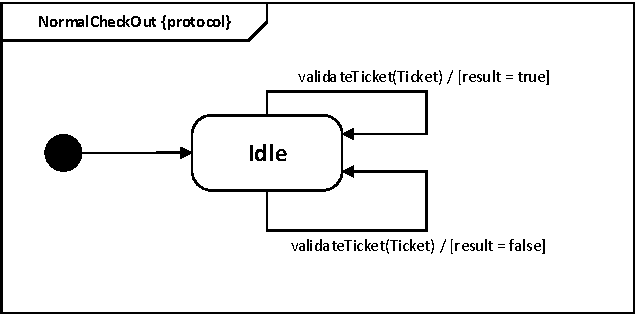
\includegraphics[width=0.7\linewidth]{img/protocol_state_machine/protocol_state_machine_station_server_to_normal_lane_check_out.png}
\caption{Interface to allow toll lanes to validate tickets}
\label{fig:protocol_state_machine_station_server_to_normal_lane_check_out}
\end{figure}

\subsection*{Station server - enterprise server}
\begin{figure}
\centering
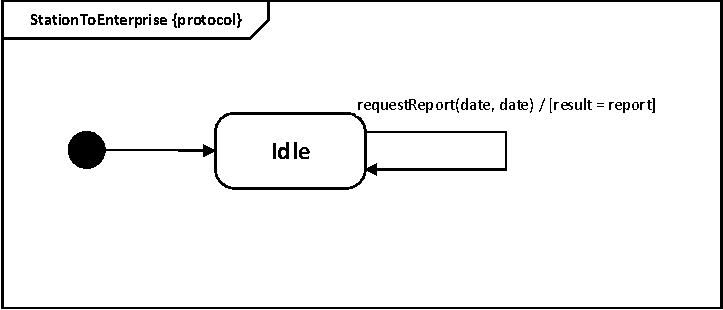
\includegraphics[width=0.7\linewidth]{img/protocol_state_machine/protocol_state_machine_station_server_to_enterprise_server.png}
\caption{Interface to use for getting data for the generation of reports}
\label{fig:protocol_state_machine_station_server_to_enterprise_server}
\end{figure}

\subsection*{Express toll lane checkout - station server}
\begin{figure}
\centering
\includegraphics[width=0.7\linewidth]{img/protocol_state_machine/protocol_state_machine_station_server with_toll_computer_check_out.png}
\caption{The communication protocol for checking out toll tag}
\label{fig:protocol_state_machine_station_server with_toll_computer_check_out}
\end{figure}

\subsection*{ticket reader}
\begin{figure}
\centering
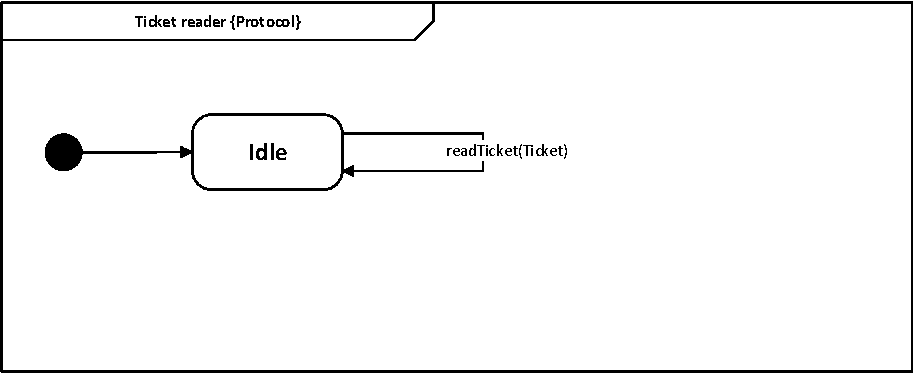
\includegraphics[width=0.7\linewidth]{img/protocol_state_machine/protocol_state_machine_ticket_reader.png}
\caption{The communication protocol for the ticket reader used during checkout for non-tag checkout}
\label{fig:protocol_state_machine_ticket_reader}
\end{figure}


\section*{Life-cycle state machines}
indsæt philip tekst